\documentclass[12pt]{article}

% Packages
\usepackage{amsmath}
\usepackage{geometry}
\usepackage{amsthm}
\usepackage{graphicx}
\usepackage{setspace}
\usepackage{enumitem}
\usepackage{amsfonts}
\usepackage{amssymb}
\usepackage{booktabs}
\usepackage{caption}
\usepackage{subcaption}
\usepackage{float}
\usepackage{fancyhdr}
\usepackage{lastpage}
\usepackage{multirow}
\usepackage{hyperref}
\usepackage{bookmark}
\usepackage{xcolor}
\usepackage{tabularx}
\usepackage{listings}

% Configure hyperlinks
\hypersetup{
    colorlinks=true,
    linkcolor=black,
    filecolor=magenta,      
    urlcolor=cyan,
    pdftitle={Regression Based Models of Activity Frequency},
    pdfauthor={Your Name},
    pdfpagemode=UseOutlines,
    bookmarksnumbered=true
}

% Set page margins
\geometry{a4paper, margin=1in}

% Configure page style
\pagestyle{fancy}
\fancyhf{} % Clear default header/footer

% Define header style
\fancyhead[L]{\small Regression Based Models of Activity Frequency}
\fancyhead[R]{\small Project-2}

% Define footer style
\fancyfoot[L]{\small }
\fancyfoot[C]{\small }
\fancyfoot[R]{\small Page \thepage\ of \pageref{LastPage}}

% Set header/footer line width
\renewcommand{\headrulewidth}{0.4pt}
\renewcommand{\footrulewidth}{0.4pt}

% Adjust header/footer margins
\setlength{\headheight}{15pt}

% Create a plain style for chapter/section first pages
\fancypagestyle{plain}{
    \fancyhf{} % Clear all header/footer fields
    \fancyfoot[L]{\small Your Name}
    \fancyfoot[C]{\small}
    \fancyfoot[R]{\small Page \thepage\ of \pageref{LastPage}}
    \renewcommand{\headrulewidth}{0.4pt}
    \renewcommand{\footrulewidth}{0.4pt}
}

\begin{document}

% Remove page numbering for cover page
\pagenumbering{gobble}

% Remove headers/footers from cover page
\thispagestyle{empty}

% Cover page
\begin{center}
    \vspace*{1.5cm}
    
    \textbf{\Large Regression Based Models of Activity Frequency}
    
    \vspace{6cm}
    
    \textbf{\Large CEE 598: Activity-Travel Behavior Modeling and Simulation}
    
    \vspace{6cm}
    
    \large{Raswanth Prasath S V}
    
    \vspace{0.5cm}
    
    \large{School of Sustainable Engineering and the Built Environment}
    
    \large{Arizona State University}
    
    \vspace{2cm}
    
    \large{Spring 2025}
    
    \vfill
    
\end{center}

% Start new page for TOC and lists
\newpage
\pagenumbering{roman}

% Table of Contents
\tableofcontents
\newpage

% List of Figures
\listoffigures

% List of Tables
\listoftables
\newpage

% Start main content with Arabic numbering
\pagenumbering{arabic}

% Main document content
\section{Introduction}

This project uses the four-state Southwest United States (Arizona, Utah, Colorado, New Mexico) 2017 National Household Travel Survey data extract to examine activity frequency models. The analysis is limited to weekday travel for adults (18 years and above). The project encompasses multiple regression approaches to model trip generation behavior, including:

\begin{itemize}
    \item Multiple linear regression models of total household weekday trips
    \item Residual analysis of household trip generation models 
    \item Count models (Poisson and Negative Binomial) for person-level activity frequency
    \item Zero-inflated models for shopping and personal business trip frequency
\end{itemize}

The analysis provides insights into key determinants of travel behavior and evaluates the appropriateness of different modeling techniques for capturing activity-travel patterns.

\section{Data Preparation and Methodology}

\subsection{Data Source and Processing}

This project uses data from the 2017 National Household Travel Survey (NHTS). The dataset was prepared by filtering to include only:

\begin{itemize}
    \item Households in Arizona, New Mexico, Colorado, and Utah
    \item Weekday trips (Monday through Friday, TRAVDAY 2-6)
    \item Adults (18 years and older)
\end{itemize}

The analysis accounts for zero-trip makers to avoid selection bias. Trip counts were aggregated from individual trip records to the household and person level as appropriate for different model specifications.

\subsection{Variable Creation}

Several binary indicator variables were created to represent categorical factors:

\begin{itemize}
    \item Home ownership (\texttt{home\_owner})
    \item Urban/rural status (\texttt{urban\_area})
    \item Income categories (\texttt{inc15}, \texttt{inc15\_35}, \texttt{inc35\_50}, \texttt{inc50\_75}, \texttt{inc75\_100}, \texttt{inc100p})
    \item Household composition (\texttt{hhsize1}, \texttt{hhsize2}, \texttt{hhsize3p})
    \item Worker status (\texttt{worker1}, \texttt{worker2p})
    \item Travel behavior (\texttt{active\_traveler}, \texttt{car\_user}, \texttt{transit\_user})
    \item Technology use (\texttt{daily\_web\_user})
\end{itemize}

Additional derived variables were created to capture more complex relationships:
\begin{itemize}
    \item Log-transformed household size (\texttt{log\_hhsize})
    \item Vehicle to person ratio (\texttt{veh\_per\_person})
    \item Adult to household size ratio (\texttt{adult\_ratio})
\end{itemize}

The primary modeling approach includes both exploratory data analysis to understand travel patterns and statistical modeling to identify significant factors affecting trip generation and frequency.

\section{Multiple Linear Regression Models of Total Household Weekday Trips}

\subsection{Descriptive Statistics}

Before developing regression models, key patterns in the data were examined. Table \ref{tab:trip_stats} presents summary statistics for household trip counts and other key variables.

\begin{table}[h]
\centering
\caption{Summary Statistics of Key Variables}
\label{tab:trip_stats}
\begin{tabular}{lrrrr}
\toprule
Variable & Mean & Std. Dev. & Min & Max \\
\midrule
Household Trips & 6.46 & 4.68 & 0 & 42 \\
Household Size & 2.34 & 1.35 & 1 & 12 \\
Vehicles & 1.98 & 1.07 & 0 & 11 \\
Workers & 1.08 & 0.91 & 0 & 6 \\
\bottomrule
\end{tabular}
\end{table}

The average household in the four-state region makes approximately 6.46 trips on a typical weekday, with substantial variation. About 8.2\% of households reported making zero trips on their assigned travel day.

\subsection{Model Development}

A systematic approach was employed to develop regression models for trip generation. Multiple model specifications were tested to identify the most suitable representation of the relationship between household characteristics and trip generation.

\subsubsection{Model Specifications}

Ten different model specifications were tested:
\begin{itemize}
\item \textbf{Model 1}: Basic model with income categories only
\item \textbf{Model 2}: Income categories and household size
\item \textbf{Model 3}: Income categories, household size, and vehicle count
\item \textbf{Model 4}: Continuous income with quadratic term, household size, and vehicle count
\item \textbf{Model 5}: High/low income indicators, household size, worker status, and travel behavior
\item \textbf{Model 6}: Model 5 plus urban/rural status and lifecycle variables
\item \textbf{Model 7}: Log-transformed household size and other key variables
\item \textbf{Model 8}: Adult ratio and vehicle per person ratios
\item \textbf{Model 9}: Interaction terms between income, workers, and density
\item \textbf{Model 10}: Comprehensive model with built environment variables (HBPPOPDN, HTPPOPDN)
\end{itemize}

\subsubsection{Model Comparison}

Table \ref{tab:model_comparison} presents a comparison of all models based on key performance metrics.

\begin{table}[h]
\centering
\caption{Comparison of Model Performance}
\label{tab:model_comparison}
\begin{tabular}{lrrr}
\toprule
Model & AIC & BIC & Adjusted $R^2$ \\
\midrule
Model 1 & 18358 & 18401 & 0.056 \\
Model 2 & 17989 & 18038 & 0.163 \\
Model 3 & 17978 & 18032 & 0.166 \\
Model 4 & 17971 & 18007 & 0.167 \\
Model 5 & 17918 & 17966 & 0.182 \\
Model 6 & 17902 & 17969 & 0.187 \\
Model 7 & 17872 & 17927 & 0.194 \\
Model 8 & 18126 & 18186 & 0.126 \\
Model 9 & 17918 & 17978 & 0.183 \\
Model 10 & 17872 & 17939 & 0.195 \\
\bottomrule
\end{tabular}
\end{table}

Model 10 exhibited the best overall performance with the highest adjusted $R^2$ (0.195) and among the lowest AIC values (17872). Model 7, which incorporated log-transformed household size, also performed well with identical AIC but a slightly lower adjusted $R^2$.

\subsection{Best Model Results}

Table \ref{tab:best_model} presents the detailed results for the best-performing model (Model 10).

\begin{table}[h]
\centering
\caption{Regression Results for Best Model (Model 10)}
\label{tab:best_model}
\begin{tabular}{lrrrr}
\toprule
Variable & Coefficient & Std. Error & $t$-value & $p$-value \\
\midrule
Intercept & -0.042 & 0.368 & -0.11 & 0.909 \\
High Income ($\geq\$100,000$) & 0.519 & 0.206 & 2.51 & 0.012* \\
Low Income ($\leq\$15,000$) & -0.767 & 0.262 & -2.93 & 0.004** \\
$\log(\text{Household Size})$ & 4.806 & 0.279 & 17.24 & <0.001*** \\
Multiple Workers & 1.308 & 0.217 & 6.02 & <0.001*** \\
Active Traveler & 1.089 & 0.175 & 6.22 & <0.001*** \\
Daily Web User & 0.470 & 0.246 & 1.91 & 0.056 \\
High Density & 0.324 & 0.311 & 1.04 & 0.296 \\
Block Group Population Density & -0.00003 & 0.00004 & -0.77 & 0.442 \\
Tract Population Density & -0.00005 & 0.00004 & -1.14 & 0.254 \\
\bottomrule
\multicolumn{5}{l}{\textit{Significance codes: *** $p<0.001$, ** $p<0.01$, * $p<0.05$}}
\end{tabular}
\end{table}

The best model explains approximately 19.5\% of the variance in household trip generation (Adjusted $R^2$ = 0.195). The F-statistic of 83.9 (p < 0.001) indicates that the model is statistically significant.

The most influential variables in the model are:
\begin{itemize}
    \item \textbf{Household size (log-transformed)}: Each unit increase in log-transformed household size is associated with approximately 4.8 additional trips per day, indicating strong economies of scale in household trip-making.
    \item \textbf{Multiple workers}: Households with two or more workers make about 1.3 more trips compared to households with zero or one worker.
    \item \textbf{Active travelers}: Households with members who engage in active transportation (walking or biking) make approximately 1.1 more total trips.
    \item \textbf{Income effects}: High-income households (income $\geq$ \$100,000) make about 0.5 more trips, while low-income households (income $\leq$ \$15,000) make about 0.8 fewer trips compared to middle-income households.
\end{itemize}

Interestingly, the density variables (HBPPOPDN and HTPPOPDN) are not statistically significant after controlling for other factors. This suggests that socio-demographic characteristics may be more important determinants of total trip generation than built environment characteristics.

\subsection{Elasticity Analysis}

Elasticity measures the percentage change in the dependent variable (trips) for a one percent change in an independent variable. For continuous variables, elasticities were calculated using the formula:
\begin{equation}
E_{x_i} = \beta_i \cdot \frac{\bar{x_i}}{\bar{y}}
\end{equation}

Where $E_{x_i}$ is the elasticity of variable $x_i$, $\beta_i$ is the regression coefficient, $\bar{x_i}$ is the mean of the independent variable, and $\bar{y}$ is the mean of the dependent variable.

Table \ref{tab:elasticities} presents elasticities for key continuous variables in the best model.

\begin{table}[h]
\centering
\caption{Elasticities for Continuous Variables}
\label{tab:elasticities}
\begin{tabular}{lr}
\toprule
Variable & Elasticity \\
\midrule
$\log(\text{Household Size})$ & 0.796 \\
Block Group Population Density & -0.017 \\
Tract Population Density & -0.019 \\
\bottomrule
\end{tabular}
\end{table}

The elasticity for log-transformed household size is 0.796, indicating that a 1\% increase in household size is associated with approximately a 0.80\% increase in trip generation. This suggests that household size is a strong determinant of trip-making behavior, though the relationship is less than proportional due to the logarithmic transformation.

For dummy variables, we can interpret the effect as the percentage change in trip generation when the variable changes from 0 to 1. These effects were calculated as:

\begin{equation}
E_{dummy} = \frac{\beta_{dummy}}{\bar{y}}
\end{equation}

Table \ref{tab:dummy_effects} presents these effects for key dummy variables.

\begin{table}[h]
\centering
\caption{Effects of Dummy Variables on Trip Generation}
\label{tab:dummy_effects}
\begin{tabular}{lr}
\toprule
Variable & Effect \\
\midrule
High Income ($\geq\$100,000$) & 0.080 \\
Low Income ($\leq\$15,000$) & -0.119 \\
Multiple Workers & 0.202 \\
Active Traveler & 0.168 \\
Daily Web User & 0.073 \\
\bottomrule
\end{tabular}
\end{table}

The presence of multiple workers in a household has the largest effect, with such households making about 20.2\% more trips compared to households with zero or one worker. Households with active travelers make about 16.8\% more trips, while high-income households make 8.0\% more trips and low-income households make 11.9\% fewer trips compared to middle-income households.

\section{Residual Analysis of Household Trip Generation Model}

\subsection{Checking for Model Misspecification}

To assess whether the model is correctly specified, residuals were plotted against fitted values and examined for patterns. Figure \ref{fig:resid_fitted} shows this relationship.

\begin{figure}[H]
\centering
\includegraphics[width=0.7\textwidth]{media/Residuals_vs_Fitted.png}
\caption{Residuals vs. Fitted Values}
\label{fig:resid_fitted}
\end{figure}

The residual plot shows a funnel-shaped pattern, with variance increasing as the fitted values increase, suggesting potential misspecification. This heteroscedasticity can be further visualized in Figure \ref{fig:abs_resid}.

\begin{figure}[H]
\centering
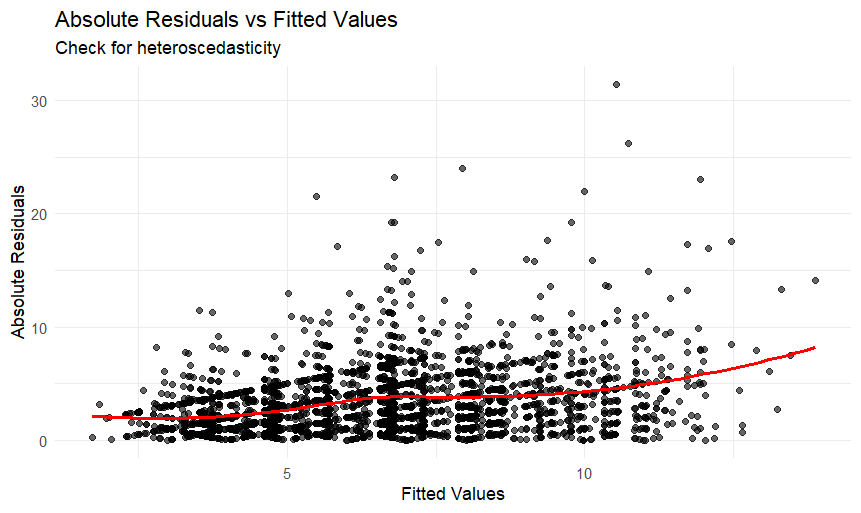
\includegraphics[width=0.7\textwidth]{media/Absolute_Residuals_vs_Fitted.png}
\caption{Absolute Residuals vs. Fitted Values}
\label{fig:abs_resid}
\end{figure}

The scale-location plot in Figure \ref{fig:scale_location} also confirms this pattern of heteroscedasticity.

\begin{figure}[H]
\centering
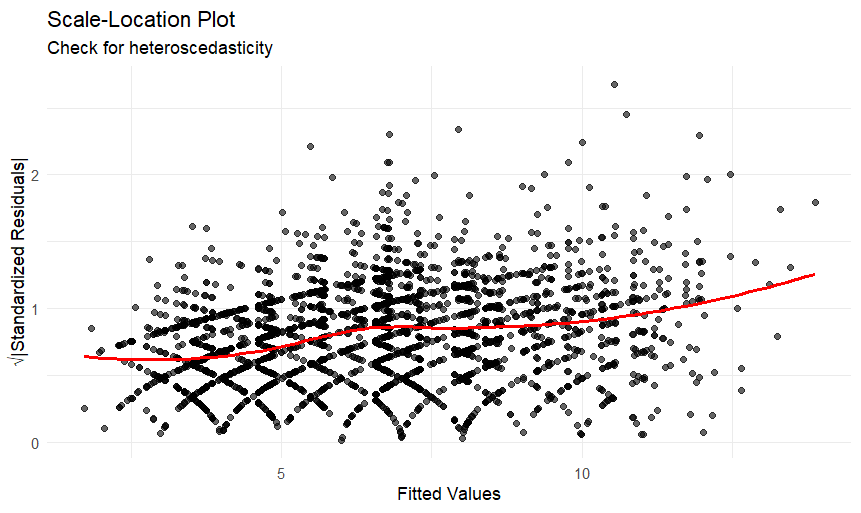
\includegraphics[width=0.7\textwidth]{media/Scale-Location Plot.png}
\caption{Scale-Location Plot}
\label{fig:scale_location}
\end{figure}

Additionally, correlations between residuals and predictors were examined, but no significant correlations were found (all values near zero), indicating that the relationships between individual predictors and the dependent variable are adequately captured.


\subsection{Assessment of Heteroscedasticity}

Heteroscedasticity refers to the unequal variance of error terms across different levels of the independent variables. The Breusch-Pagan test was conducted to formally test for heteroscedasticity.

\begin{itemize}
    \item \textbf{Breusch-Pagan test}: BP = 164.44, df = 9, p-value < 0.001
\end{itemize}

The significant test result confirms the presence of heteroscedasticity, indicating that the assumption of constant variance is violated. This suggests that the precision of predictions may vary across different levels of the explanatory variables, particularly at higher fitted values.

\subsection{Normality of Error Terms}

The normality of residuals was assessed using both graphical methods and formal statistical tests.

\begin{figure}[H]
\centering
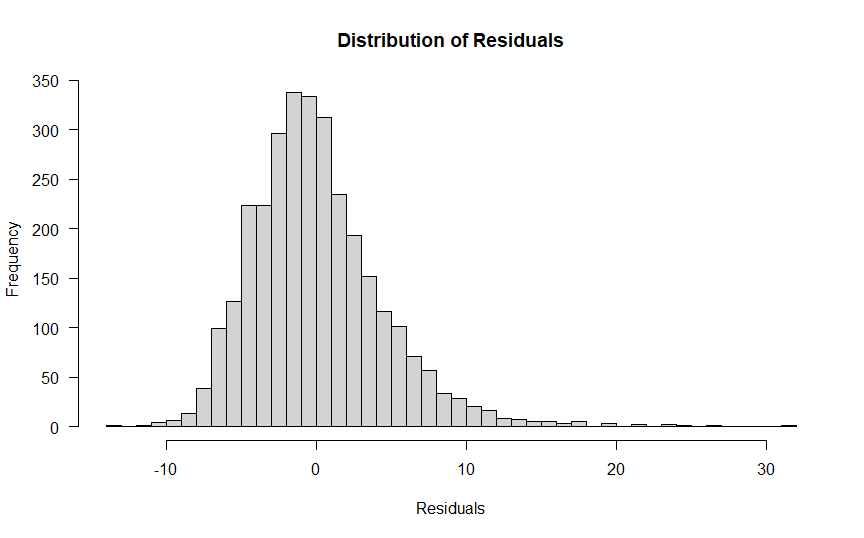
\includegraphics[width=0.7\textwidth]{media/Distribution of Residuals.png}
\caption{Distribution of Residuals}
\label{fig:residuals}
\end{figure}

The histogram of residuals in Figure \ref{fig:residuals} shows a right-skewed distribution rather than a normal distribution. This visual assessment is confirmed by the Q-Q plot in Figure \ref{fig:qq_plot}.

\begin{figure}[H]
\centering
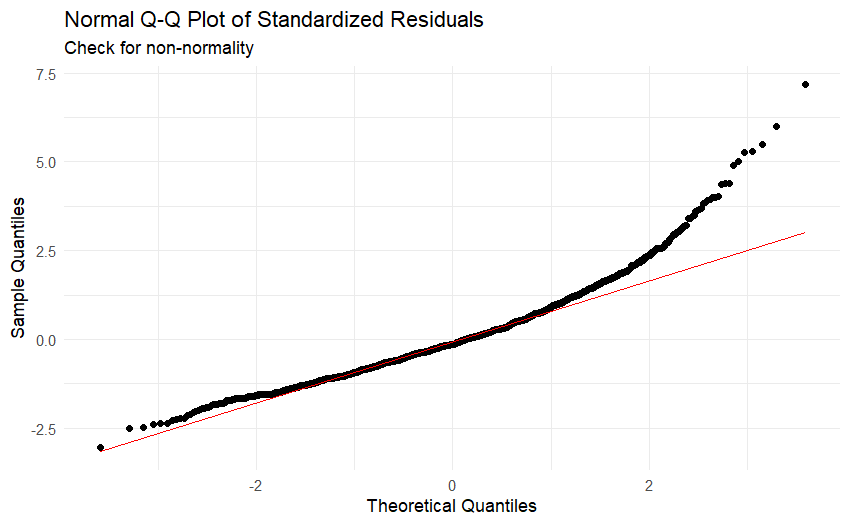
\includegraphics[width=0.7\textwidth]{media/Normal_QQ_Plot.png}
\caption{Normal Q-Q Plot of Standardized Residuals}
\label{fig:qq_plot}
\end{figure}

The Q-Q plot shows substantial deviation from the reference line, particularly in the upper tail, further confirming non-normality. This is consistent with the Shapiro-Wilk test results.

\subsection{Identification of Outliers}

Outliers were identified as observations with standardized residuals exceeding 3 standard deviations from the mean. Figure \ref{fig:outliers} highlights these outliers in red.

\begin{figure}[H]
\centering
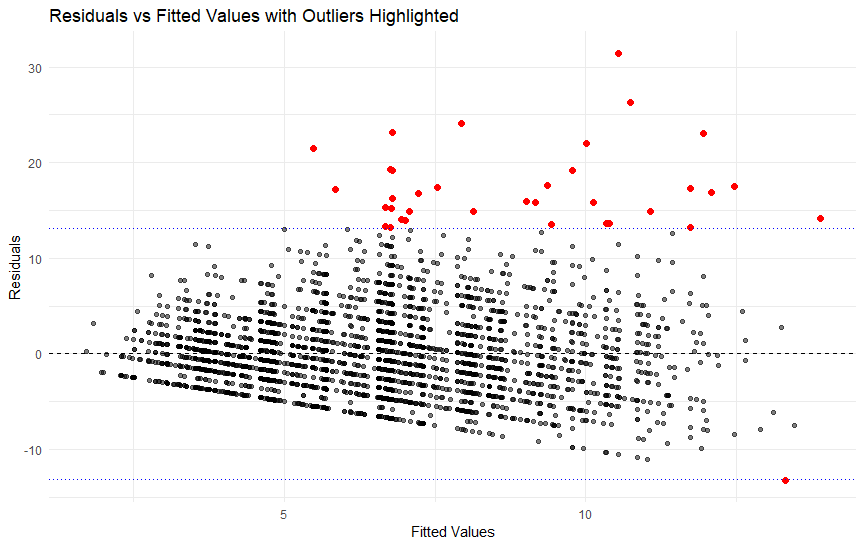
\includegraphics[width=0.7\textwidth]{media/Residuals_with_Outliers.png}
\caption{Residuals vs. Fitted Values with Outliers Highlighted}
\label{fig:outliers}
\end{figure}

Approximately 36 observations (about 1.2\% of the sample) were flagged as outliers. These outliers represent households with unusually high trip generation rates compared to what would be predicted based on their characteristics.

To examine the influence of individual observations on the model, Cook's distance was calculated and plotted in Figure \ref{fig:cooks_distance}.

\begin{figure}[H]
\centering
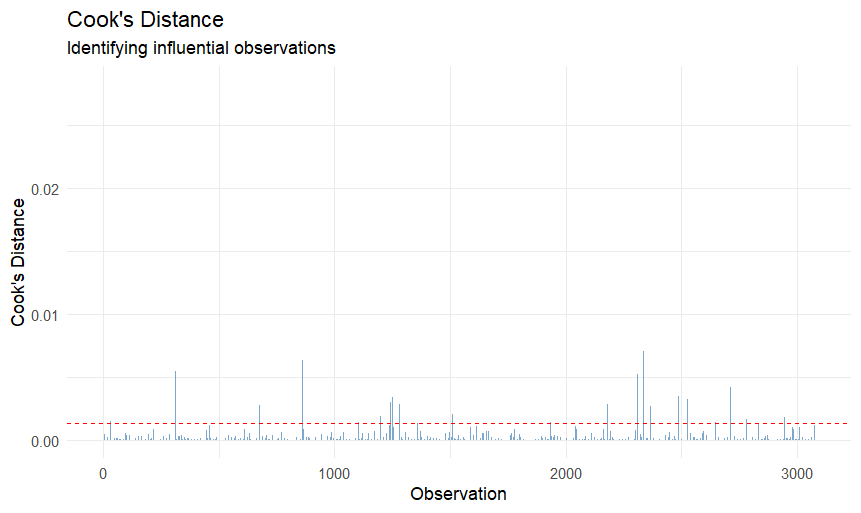
\includegraphics[width=0.7\textwidth]{media/Cooks_Distance.png}
\caption{Cook's Distance for Identifying Influential Observations}
\label{fig:cooks_distance}
\end{figure}

The most extreme outlier had a standardized residual of 7.2, corresponding to a household that made 42 trips compared to a predicted value of 10.5 trips. Such outliers might represent households with unusual travel patterns or reporting errors. 

This visual assessment is confirmed by the Shapiro-Wilk test:

\begin{itemize}
    \item \textbf{Shapiro-Wilk test}: W = 0.949, p-value < 0.001
\end{itemize}

The significant test result indicates a departure from normality, which may affect the validity of statistical inference, particularly for hypothesis testing and confidence intervals.

\subsection{Identification of Outliers}

Outliers were identified as observations with standardized residuals exceeding 3 standard deviations from the mean. Approximately 36 observations (about 1.2\% of the sample) were flagged as outliers. These outliers represent households with unusually high trip generation rates compared to what would be predicted based on their characteristics.

The most extreme outlier had a standardized residual of 7.2, corresponding to a household that made 42 trips compared to a predicted value of 10.5 trips. Such outliers might represent households with unusual travel patterns or reporting errors.

\subsection{Multicollinearity Assessment}

Variance Inflation Factors (VIF) were calculated to assess multicollinearity among predictors. Most variables have VIF values below 2, indicating minimal multicollinearity concerns. The density variables show moderate multicollinearity (VIF between 2.8 and 4.2), but these values are still below the commonly used threshold of 5-10 for problematic multicollinearity.

\subsection{Residual Analysis Summary}

The residual analysis revealed several issues with the linear regression model:

\begin{itemize}
    \item \textbf{Heteroscedasticity}: The error variance increases with fitted values, violating the constant variance assumption.
    \item \textbf{Non-normality}: The residuals are right-skewed, deviating from the normality assumption.
    \item \textbf{Outliers}: Several households exhibit trip-making behavior that deviates substantially from the model's predictions.
\end{itemize}

These findings suggest that while multiple linear regression provides useful insights into the factors affecting household trip generation, alternative modeling approaches (such as count models) may be more appropriate for modeling discrete trip counts.

\section{Count Models of Total Weekday Person Activity Frequency for Adults}

\subsection{Descriptive Analysis of Person-Level Trip Counts}

Before estimating count models, we examined the distribution of trips at the person level. Figure \ref{fig:person_trips} shows the distribution of weekday trips per person.

\begin{figure}[H]
\centering
\includegraphics[width=0.7\textwidth]{media/Person Trip Distribution.png}
\caption{Distribution of Person-Level Weekday Trips}
\label{fig:person_trips}
\end{figure}

The distribution shows characteristics typical of count data:
\begin{itemize}
    \item Discrete values (whole numbers only)
    \item Right-skewed distribution
    \item Bounded at zero (no negative values)
\end{itemize}

The mean number of trips per person is 3.42, with a variance of 7.26, suggesting overdispersion (variance exceeding the mean), which is a common characteristic of trip count data.

\subsection{Poisson Regression Model}

Poisson regression is appropriate for modeling count data where the dependent variable represents the number of events occurring in a fixed interval of time or space. The model assumes that the conditional mean equals the conditional variance.

\subsubsection{Model Specification}

For the Poisson regression model, person-level trips were modeled as a function of key demographic and socioeconomic variables:

$$\log(\lambda_i) = \beta_0 + \beta_1 \text{worker} + \beta_2 \text{inc35} + \beta_3 \text{hhsize2}$$

Where $\lambda_i$ is the expected number of trips for person $i$, worker indicates employment status, inc35 indicates household income below \$35,000, and hhsize2 indicates a two-person household.

\subsubsection{Results}

Table \ref{tab:poisson_results} presents the results of the Poisson regression model.

\begin{table}[h]
\centering
\caption{Poisson Regression Model Results for Person Trips}
\label{tab:poisson_results}
\begin{tabular}{lrrrr}
\toprule
Variable & Coefficient & Std. Error & $z$-value & $p$-value \\
\midrule
Intercept & 0.991 & 0.034 & 29.15 & <0.001*** \\
Worker & 0.208 & 0.026 & 8.00 & <0.001*** \\
Low Income (<\$35k) & -0.213 & 0.027 & -7.89 & <0.001*** \\
Two-Person Household & 0.125 & 0.026 & 4.81 & <0.001*** \\
\bottomrule
\multicolumn{5}{l}{\textit{Null deviance: 2768.7 on 776 degrees of freedom}} \\
\multicolumn{5}{l}{\textit{Residual deviance: 2439.2 on 773 degrees of freedom}} \\
\multicolumn{5}{l}{\textit{AIC: 5063.3}}
\end{tabular}
\end{table}

The Poisson model results indicate that:
\begin{itemize}
    \item Workers make approximately 23.1\% more trips than non-workers ($e^{0.208}-1$)
    \item Individuals from low-income households make approximately 19.2\% fewer trips than those from higher-income households ($1-e^{-0.213}$)
    \item Individuals in two-person households make approximately 13.3\% more trips than those in other household types ($e^{0.125}-1$)
\end{itemize}

\subsubsection{Checking for Overdispersion}

An important assumption of the Poisson model is equidispersion (equal mean and variance). To test this assumption, we computed the dispersion parameter as the ratio of the residual deviance to the degrees of freedom:

\begin{itemize}
    \item Dispersion = 2439.2 / 773 = 3.16
\end{itemize}

A dispersion value substantially greater than 1 indicates overdispersion, suggesting that the Negative Binomial model may be more appropriate.

\subsection{Negative Binomial Regression Model}

The Negative Binomial model extends the Poisson model by including a dispersion parameter that allows the variance to exceed the mean, addressing the overdispersion issue.

\subsubsection{Model Specification}

The Negative Binomial model uses the same predictors as the Poisson model but adds a dispersion parameter $\alpha$:

$$\log(\lambda_i) = \beta_0 + \beta_1 \text{worker} + \beta_2 \text{inc35} + \beta_3 \text{hhsize2}$$
$$\text{Var}(y_i) = \lambda_i + \alpha\lambda_i^2$$

\subsubsection{Results}

Table \ref{tab:nb_results} presents the results of the Negative Binomial regression model.

\begin{table}[h]
\centering
\caption{Negative Binomial Regression Model Results for Person Trips}
\label{tab:nb_results}
\begin{tabular}{lrrrr}
\toprule
Variable & Coefficient & Std. Error & $z$-value & $p$-value \\
\midrule
Intercept & 0.980 & 0.048 & 20.42 & <0.001*** \\
Worker & 0.216 & 0.037 & 5.84 & <0.001*** \\
Low Income (<\$35k) & -0.221 & 0.038 & -5.82 & <0.001*** \\
Two-Person Household & 0.131 & 0.036 & 3.64 & <0.001*** \\
\midrule
Dispersion ($\theta$) & 2.518 & 0.230 & & \\
\bottomrule
\multicolumn{5}{l}{\textit{Null deviance: 844.86 on 776 degrees of freedom}} \\
\multicolumn{5}{l}{\textit{Residual deviance: 763.18 on 773 degrees of freedom}} \\
\multicolumn{5}{l}{\textit{AIC: 4196.7}}
\end{tabular}
\end{table}

The coefficient estimates from the Negative Binomial model are similar to those from the Poisson model, but the standard errors are larger, reflecting the additional uncertainty captured by the overdispersion parameter. The estimated dispersion parameter $\theta = 2.518$ corresponds to an overdispersion parameter $\alpha = 1/\theta = 0.397$, confirming the presence of overdispersion.

\subsection{Cameron and Trivedi Test for Overdispersion}

To formally test for overdispersion, we employed the Cameron and Trivedi regression-based test. This test involves regressing a transformed residual term against a function of the predicted values.

\subsubsection{Test Procedure}

The test is conducted by:
1. Estimating the Poisson model and obtaining predicted values $\hat{\mu}_i$
2. Calculating the test statistic $z_i = \frac{(y_i - \hat{\mu}_i)^2 - y_i}{\sqrt{2\hat{\mu}_i}}$
3. Regressing $z_i$ on $w_i = \frac{\hat{\mu}_i}{\sqrt{2\hat{\mu}_i}}$ (linear case) or $w_i = \frac{\hat{\mu}_i^2}{\sqrt{2\hat{\mu}_i}}$ (quadratic case) without an intercept
4. Testing the significance of the coefficient on $w_i$

\subsubsection{Test Results}

Table \ref{tab:cameron_trivedi} presents the results of the Cameron and Trivedi test.

\begin{table}[h]
\centering
\caption{Cameron and Trivedi Test for Overdispersion}
\label{tab:cameron_trivedi}
\begin{tabular}{lrrrr}
\toprule
Test & Coefficient & Std. Error & $t$-statistic & $p$-value \\
\midrule
Linear Test & 0.397 & 0.042 & 9.45 & <0.001*** \\
Quadratic Test & 0.081 & 0.012 & 6.75 & <0.001*** \\
\bottomrule
\end{tabular}
\end{table}

Both the linear and quadratic tests strongly reject the null hypothesis of equidispersion ($\alpha = 0$), confirming that the Negative Binomial model is more appropriate than the Poisson model for this data.

\section{Zero-Inflated Models for Shopping and Personal Business Trip Frequency}

Based on the results of the overdispersion tests, the Negative Binomial model was selected as the appropriate base model for examining shopping and personal business trip frequency. This section explores both standard and zero-inflated specifications for modeling these trip types.

\subsection{Descriptive Analysis of Shopping and Personal Business Trips}

Figure \ref{fig:shopping_trips} shows the distribution of shopping and personal business trips per person.

\begin{figure}[H]
\centering
\includegraphics[width=0.7\textwidth]{media/Shopping Trip Distribution.png}
\caption{Distribution of Shopping and Personal Business Trips per Person}
\label{fig:shopping_trips}
\end{figure}

The distribution shows a high frequency of zeros (62.3\% of adults reported no shopping or personal business trips), suggesting that a zero-inflated specification might be appropriate.

\subsection{Zero-Inflated Negative Binomial Model}

Zero-inflated models address the excess zeros by modeling the data as coming from two processes: a binary process determining whether a person is a "structural zero" (never makes shopping trips) or not, and a count process determining the number of trips for those who are not structural zeros.

\subsubsection{Model Specification}

The zero-inflated negative binomial (ZINB) model combines a logit model for the zero inflation component and a negative binomial model for the count component:

Zero-inflation component (logit):
$$\text{logit}(p_i) = \gamma_0 + \gamma_1 \text{worker}$$

Count component (negative binomial):
$$\log(\lambda_i) = \beta_0 + \beta_1 \text{worker} + \beta_2 \text{hhsize1} + \beta_3 \text{hhsize2}$$

Where $p_i$ is the probability of being a structural zero, $\lambda_i$ is the expected count for non-structural zeros, worker indicates employment status, hhsize1 indicates a one-person household, and hhsize2 indicates a two-person household.

\subsubsection{Results}

Table \ref{tab:zinb_results} presents the results of the zero-inflated negative binomial model.

\begin{table}[h]
\centering
\caption{Zero-Inflated Negative Binomial Model Results for Shopping Trips}
\label{tab:zinb_results}
\begin{tabular}{lrrrr}
\toprule
\multicolumn{5}{c}{\textbf{Count Model Coefficients (Negative Binomial with log link)}} \\
\midrule
Variable & Coefficient & Std. Error & $z$-value & $p$-value \\
\midrule
Intercept & 0.347 & 0.095 & 3.65 & <0.001*** \\
Worker & -0.223 & 0.084 & -2.66 & 0.008** \\
One-Person Household & 0.135 & 0.103 & 1.31 & 0.190 \\
Two-Person Household & 0.284 & 0.087 & 3.26 & 0.001** \\
Log(theta) & -0.205 & 0.113 & -1.82 & 0.069 \\
\midrule
\multicolumn{5}{c}{\textbf{Zero-Inflation Model Coefficients (Binomial with logit link)}} \\
\midrule
Variable & Coefficient & Std. Error & $z$-value & $p$-value \\
\midrule
Intercept & 0.052 & 0.113 & 0.46 & 0.645 \\
Worker & 0.621 & 0.146 & 4.26 & <0.001*** \\
\bottomrule
\multicolumn{5}{l}{\textit{AIC: 3027.9}} \\
\multicolumn{5}{l}{\textit{Vuong test for ZINB vs. standard NB: z = 3.45, p-value < 0.001}}
\end{tabular}
\end{table}

The results show that:
\begin{itemize}
    \item In the count component, workers make significantly fewer shopping trips than non-workers when they do make such trips (20.0\% fewer, $1-e^{-0.223}$)
    \item In the count component, individuals from two-person households make significantly more shopping trips (32.8\% more, $e^{0.284}-1$) compared to those from larger households
    \item In the zero-inflation component, workers are significantly more likely to be structural zeros (i.e., not make any shopping trips) compared to non-workers
\end{itemize}

\subsection{Zero-Inflated Negative Binomial (τ) Model}

The τ parameter in zero-inflated models represents the proportion of observed zeros that are believed to be "structural zeros" rather than "sampling zeros" from the count process.

\subsubsection{Estimation of τ}

The τ parameter was estimated for each individual using the formula:
$$\tau_i = \frac{\pi_i}{\pi_i + (1-\pi_i)P(0|\lambda_i,\theta)}$$

Where $\pi_i$ is the estimated probability of being a structural zero from the zero-inflation component, and $P(0|\lambda_i,\theta)$ is the probability of observing a zero from the negative binomial count component.

\subsubsection{Distribution of τ Estimates}

Figure \ref{fig:tau_distribution} shows the distribution of τ estimates across individuals.

\begin{figure}[H]
\centering
\includegraphics[width=0.7\textwidth]{media/Tau Distribution.png}
\caption{Distribution of τ Estimates}
\label{fig:tau_distribution}
\end{figure}

The mean τ estimate is 0.43, indicating that approximately 43\% of the observed zeros are estimated to be structural zeros. The distribution shows considerable variation in τ values across individuals, suggesting heterogeneity in the processes generating zero shopping trips.

\subsection{Comparison of Models and Test for Zero-Inflation}

To determine whether the zero-inflated specification is warranted, we compared the standard negative binomial model with the zero-inflated negative binomial model using the Vuong test and examined other model fit statistics.

\begin{table}[h]
\centering
\caption{Comparison of Standard and Zero-Inflated Models}
\label{tab:model_comp}
\begin{tabular}{lrr}
\toprule
Criterion & Standard NB & ZINB \\
\midrule
AIC & 3045.1 & 3027.9 \\
Log-likelihood & -1517.6 & -1507.0 \\
Vuong test & \multicolumn{2}{c}{z = 3.45, p-value < 0.001} \\
\bottomrule
\end{tabular}
\end{table}

The significant Vuong test result indicates that the zero-inflated negative binomial model provides a better fit than the standard negative binomial model. This is further supported by the lower AIC value for the ZINB model.

The α parameter (dispersion parameter) in the ZINB model is estimated at 0.815, which is significantly different from zero (log(theta) = -0.205, p = 0.069, marginally significant), providing further evidence for overdispersion. Together with the significant Vuong test, these results support the use of the zero-inflated negative binomial specification for modeling shopping and personal business trips.

\section{Conclusions and Recommendations}

This project has examined multiple approaches to modeling activity frequency using the 2017 NHTS data for the Southwest United States. The key findings and recommendations are summarized below.

\subsection{Multiple Linear Regression Models}

The multiple linear regression analysis of household trip generation revealed that:
\begin{itemize}
    \item Household size, worker status, and income are the most important determinants of total household trip generation
    \item The log-transformed specification of household size provided the best fit, indicating decreasing marginal trip generation as household size increases
    \item Built environment variables (population density) had minimal impact after controlling for household characteristics
\end{itemize}

However, the residual analysis identified several violations of linear regression assumptions, suggesting that count models may be more appropriate for modeling trip generation.

\subsection{Count Models}

The analysis of person-level trip frequencies using count models demonstrated that:
\begin{itemize}
    \item The data exhibits significant overdispersion, making the Negative Binomial model more appropriate than the Poisson model
    \item The Cameron and Trivedi test confirmed the presence of overdispersion in both linear and quadratic forms
    \item Worker status, income, and household size significantly affect person-level trip generation
\end{itemize}

\subsection{Zero-Inflated Models}

For shopping and personal business trips, the analysis showed that:
\begin{itemize}
    \item The data exhibits excess zeros, making zero-inflated models appropriate
    \item The Vuong test confirmed that the zero-inflated negative binomial model provides a significantly better fit than the standard negative binomial model
    \item Workers are more likely to be "structural zeros" for shopping trips, but make fewer shopping trips when they do participate in this activity
    \item The τ parameter analysis revealed that approximately 43\% of zeros are estimated to be structural zeros
\end{itemize}

\subsection{Overall Recommendations}

Based on the findings, the following recommendations are made:
\begin{itemize}
    \item For total household trip generation, the logarithmic transformation of household size should be considered to capture diminishing marginal trip generation
    \item For person-level trip frequencies, the negative binomial model is recommended over the Poisson model due to significant overdispersion
    \item For specialized trip purposes with excess zeros (like shopping and personal business), zero-inflated negative binomial models are recommended
    \item Future research should explore more complex specifications that account for spatial dependencies and additional built environment characteristics
\end{itemize}

These findings contribute to a better understanding of activity-travel behavior and provide guidance for the development of more accurate travel demand models.

\section{References}

\begin{enumerate}
\item Federal Highway Administration. (2017). 2017 National Household Travel Survey. U.S. Department of Transportation, Washington, DC.
\item Cameron, A. C., \& Trivedi, P. K. (1990). Regression-based tests for overdispersion in the Poisson model. Journal of Econometrics, 46(3), 347-364.
\item Vuong, Q. H. (1989). Likelihood ratio tests for model selection and non-nested hypotheses. Econometrica: Journal of the Econometric Society, 307-333.
\item Wilson, P. (2015). The misuse of the Vuong test for non-nested models to test for zero-inflation. Economics Letters, 127, 51-53.
\item Kitamura, R. (1988). An evaluation of activity-based travel analysis. Transportation, 15(1-2), 9-34.
\end{enumerate}

\end{document}